

\subsection*{Volume por Fatiamento}
\begin{frame}
\frametitle{Volumes por fatiamento}


Uma \dt{seção transversal } de um sólido $S$ é a região plana formada pela interseção entre $S$ e um plano. Seja $S$ um sólido limitado por dois planos perpendiculares a um eixo $OX$ nos pontos $a$ e $b$. Se $A:[a,b]\to \R$ é a função contínua que para cada $x\in[a,b]$ associa a área $A(x)$ da seção transversal de $S$ por um plano perpendicular a $OX$ no ponto $x$, então podemos aproximar o volume do sólido $S$. 

\begin{center}
\includegraphics[scale=0.4]{volume-fatia.png}
\end{center}




\end{frame}



\begin{frame}
\begin{itemize}
\item $P=\{a=x_0,x_1,\cdots,x_n=b\}$ uma partição de $[a,b]$.
\item $S$ é divido em $n$ ``fatias'' de largura $\Delta x_k$.
\item $\{x_1^\ast,x_2^\ast,\cdots,x_n^\ast\}$ um pontilhamento da partição $P$ 
\end{itemize}

%Seja $P=\{a=x_0,x_1,\cdots,x_n=b\}$ uma partição de $[a,b]$. Os planos $P_{x_k}$ perpendiculares a $OX$ dividem $S$ em $n$ ``fatias'' de largura $\Delta x_k$. Dado um pontilhamento $\{c_1,c_2,\cdots,c_n\}$ da partição $P$ podemos ver que o volume de cada fatia $V_k$ é aproximadamente
%\[V_k\approx A(c_i)\Delta x_k.\]

\begin{center}
\includegraphics[scale=0.37]{volume-fatia-particao.png}
\end{center}

\[V_i\approx A(x_i^\ast)\Delta x_i.\]

\end{frame}

\begin{frame}

Portanto o volume $V$ do sólido $S$ é aproximadamente
\[V\approx\sum_{k=1}^n A(x_i^\ast)\Delta x_i.\]
Com isso, aplicando o limite quando $\|P\|\to 0$ temos que
\[V=\lim_{\|P\|\to 0}\sum_{k=1}^n A(x_i^\ast)\Delta x_i=\int_a^bA(x)dx.\] 

\end{frame}



\begin{frame}

\begin{exe}

Uma cunha curva foi obtida por meio do corte da metade de um cilindro de raio 4 por dois planos. Um deles é perpendicular ao eixo do cilindro. O segundo cruza o primeiro, formando um ângulo de $30^\circ$ no centro do cilindro. determine o volume da cunha.

\end{exe}


\begin{center}
\includegraphics[scale=.7]{figuras/cunha.png}
\end{center}

\end{frame}


\subsection*{Sólidos de Revolução}
\begin{frame}{Sólidos de Revolução \includegraphics[scale=0.015]{figuras/fist.png}}\label{current}
\begin{center}
\includegraphics[scale=.4]{figuras/solidos-revolucao.png}
\end{center}
\end{frame}



\subsection*{Sólidos de Revolução: Método dos Discos}
\begin{frame}{Método dos Discos}
No caso em que o eixo de rotação é {\color{blue}paralelo} ao eixo de coordenadas, podemos usar o chamado {\color{blue} método dos discos}.

\[V=\int_a^b \pi \left(f(x)\right)^2\,dx\]

\begin{center}
\includegraphics[scale=.4]{figuras/discos1.png}
\end{center}
\end{frame}

\begin{frame}
\begin{exe}
Mostre que o volume da esfera de raio $r$ é $\frac{4}{3}\pi r^3$.
\end{exe}

\begin{center}
\includegraphics[scale=.7]{figuras/esfera.png}
\end{center}
\end{frame}

\begin{frame}
Usando o mesmo raciocínio, podemos resolver o seguinte tipo de problema:

\[V=\int_a^b \pi \left[\left(f(x)\right)^2-\left(g(x)\right)^2\right]\,dx\]

\begin{center}
\begin{minipage}{0.45\textwidth}
\includegraphics[scale=.5]{figuras/arruela1.png}
\end{minipage}
\begin{minipage}{0.45\textwidth}
\includegraphics[scale=.5]{figuras/arruela2.png}
\end{minipage}
\end{center}
\end{frame}



\subsection*{Sólidos de revolução: Método das Cascas Cilíndricas}
\begin{frame}
\frametitle{Volume por cascas cilíndricas }
%\begin{small}

\uncover<1->{Sejam $f:[a,b]\to \R$ uma função contínua não negativa com $a>0$. Considere a região limitada pelo gráfico de $f$ e o eixo $OX$. Ao girarmos essa região em torno do eixo $OY$ geramos um sólido $S$. 

\begin{center}
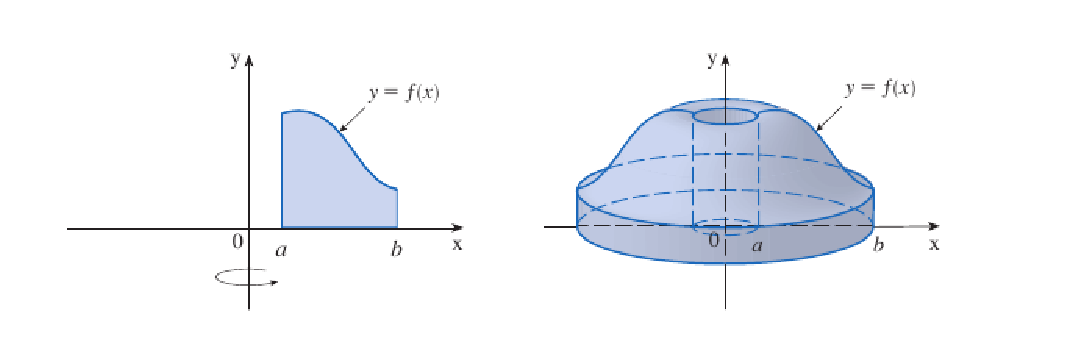
\includegraphics[scale=0.7]{casca1.eps}

\end{center}
}

%\end{small}
\end{frame}


\begin{frame}
\frametitle{ }
\begin{small}

\uncover<1->{
\begin{itemize}
\item $P=\{a=x_0,\ldots,x_n=b\}$  partição de $[a,b]$ 
\item $C=\{\overline{x}_1,\overline{x}_2,\ldots,\overline{x}_n\}$ um pontilhamento de $P$, onde $\overline{x}_i=\frac{x_{i-1}+x_i}{2}$  
\end{itemize}
\begin{center}
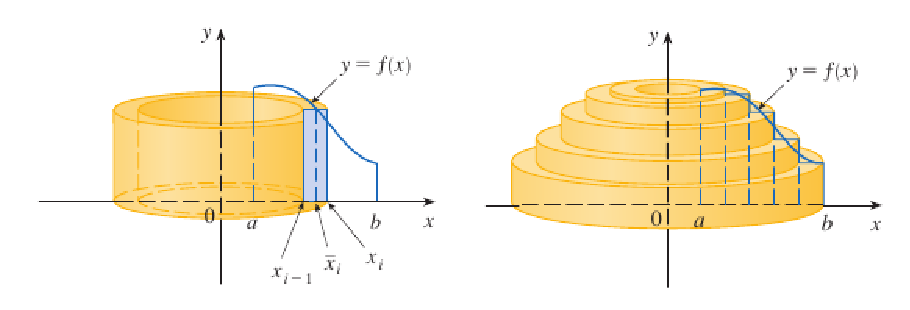
\includegraphics[scale=0.8]{casca3.eps}
\end{center} 

Com isso, o volume do sólido é dado por
$$V=2\pi\int_a^b xf(x)dx $$}

\end{small}
\end{frame}


\begin{frame}
\frametitle{ }
\uncover<1->{\begin{exe}
Calcule o volume do sólido obtido pela rotação em torno do eixo y da região limitada por $y=2x^2-x^3$ e $y=0$.

%\item Ache o volume do sólido obtido pela rotação em torno do eixo y da região entre $y=x$ e $y=x^2$.
\end{exe} }


\begin{minipage}{0.5\textwidth}
\includegraphics[scale=0.6]{figuras/solido-cascas-clindricas1.png}
\end{minipage}
\begin{minipage}{0.4\textwidth}
\includegraphics[scale=0.5]{figuras/solido-cascas-clindricas2.png}
\end{minipage}

\end{frame}

%\begin{frame}
%
%
%\uncover<1->{\begin{casa} Usando o método das cascas cilíndricas determine o volume do sólido gerado pela rotação da região limitada pela curva $y=\sqrt{x}$ e  pelas retas $y=1$ e $x=4$ em torno do eixo $y=-1$.
%\medskip
%
%\textbf{Resposta: $\frac{47\pi}{6}$}
%\end{casa}} 
%
%\end{frame}


\begin{frame}
\begin{casa}

\begin{enumerate}
%\item Mostre que o volume da pirâmide cuja altura é $h$ e base quadrada com lado $a$ é $\frac{1}{3}a^2h$.

\item Encontre o volume do sólido obtido pela rotação em torno do exio $x$ da região limitada  pelas curvas $y=x$ e $y=x^2$.

\includegraphics[scale=0.4]{figuras/arruela3.png}

\item Encontre o volume do sólido obtido pela rotação da região limitada por $y=x-x^2$ e $y=0$ em torno da reta $x=2$.

%\item Determine o volume do sólido obtido pela rotação em torno do eixo $x$ da região limitada pela curva $y=x^2+1$ e pela reta $y=-x+3$. (resposta: $117\pi/5$)
\end{enumerate}

\end{casa}
\end{frame}

\subsection*{Comprimento de Curvas}


\begin{frame}{Comprimento de Curvas}
%
\only<1>{Imagine que se queira calcular o comprimento da curva do gráfico abaixo.}
\only<2>{Uma aproximação seria o comprimento do seguimento ligando os extremos da curva.}
\only<3>{Podemos melhorar a aproximação considerando o comprimento de uma poligonal.}
\only<4>{Quanto mais divisões, melhor a aproximação!}

\begin{center}
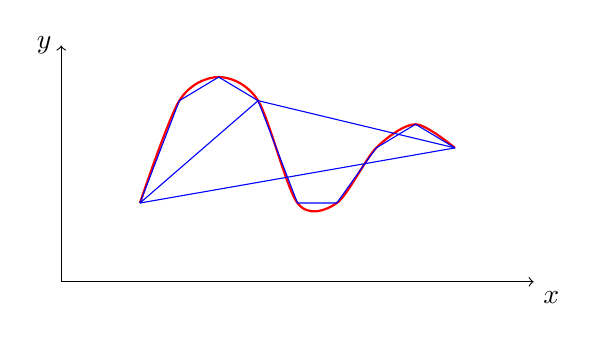
\begin{tikzpicture}
\draw[->](0,0)--(6,0) node[below right] {$x$};
\draw[->](0,0)--(0,3)node[left] {$y$};
\draw[red,thick] plot [smooth] coordinates {(1,1)(1.5,2.3)(2,2.6)(2.5,2.3)(3,1)(3.5,1)(4,1.7)(4.5,2)(5,1.7)};

\draw<2>[blue] (1,1) -- (5,1.7);

\draw<3>[blue](1,1)--(2.5,2.3)--(5,1.7);

\draw<4>[blue] (1,1)--(1.5,2.3)--(2,2.6)--(2.5,2.3)--(3,1)--(3.5,1)--(4,1.7)--(4.5,2)--(5,1.7);
\end{tikzpicture}
\end{center}
%
%
\end{frame}
%


\begin{frame}


Assim, seja \textcolor{red}{$f:[a,b]\to \R$} uma função, a fim de calcular uma aproximação do comprimento da curva dada pelo gráfico de $f$ subdividimos o intervalo $[a,b]$ em vários subintervalos e calculamos o comprimento da \textcolor{blue}{poligonal}, como abaixo.

\begin{center}
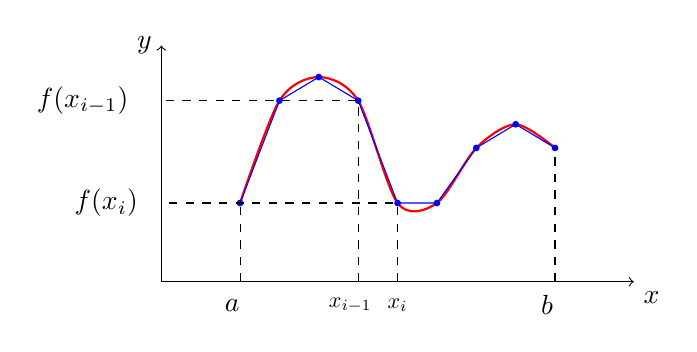
\begin{tikzpicture}
\draw[->](0,0)--(6,0) node[below right] {$x$};
\draw[->](0,0)--(0,3)node[left] {$y$};
%\psdots(1,0)(5,0)
\draw[red,thick] plot [smooth] coordinates {(1,1)(1.5,2.3)(2,2.6)(2.5,2.3)(3,1)(3.5,1)(4,1.7)(4.5,2)(5,1.7)};
\draw[blue] plot [mark=*,mark size=1] coordinates {(1,1)(1.5,2.3)(2,2.6)(2.5,2.3)(3,1)(3.5,1)(4,1.7)(4.5,2)(5,1.7)};
%\draw[blue] (1,1)--(1.5,2.3)--(2,2.6)--(2.5,2.3)--(3,1)--(3.5,1)--(4,1.7)--(4.5,2)--(5,1.7);
\draw[dashed](2.5,0)--(2.5,2.3)--(0,2.3);
\draw[dashed](3,0)--(3,1)--(0,1);
%\psdots(1,0)(1.5,0)(2,0)(2.5,0)(3,0)(3.5,0)(4,0)(4.5,0)(5,0)(0,2.3)(0,1)
\draw[dashed] (1,0) -- (1,1);
\draw[dashed] (5,0) -- (5,1.7);
\node at (0.9,-0.3) {$a$};
\node at(4.9,-0.3){$b$};
\node[scale=0.8] at(2.4,-0.3){$x_{i-1}$};
\node[scale=0.8] at(3,-0.3){$x_{i}$};
\node at(-1,2.3){$f(x_{i-1})$};
\node at(-0.7,1){$f(x_i)$};
\end{tikzpicture}
\end{center}

\[L_i=\sqrt{\Delta x_i^2+(f(x_i)-f(x_{i-1}))^2}=\sqrt{1+\left(\frac{f(x_i)-f(x_{i-1})}{\Delta x_i}\right)^2}\ \Delta x_i\]

\end{frame}
%
%
%
\begin{frame}
\frametitle{ }


Pelo Teorema do Valor Médio, existe $c_i\in [x_{i-1},x_i]$ tal que 
\[\dps\frac{f(x_i)-f(x_{i-1})}{\Delta x_i}=f'(c_i),\]
portanto,
\[L_i=\sqrt{1+(f'(c_i))^2}\ \Delta x_i\]

Com isso, o comprimento $L$ da curva é 
\[L=\lim_{\|P\|\to 0} \sum_{i=1}^n\sqrt{1+(f'(c_i))^2}\ \Delta x_i=\int_a^b\sqrt{1+(f'(x))^2}\ dx.\]

\end{frame}

\begin{frame}



\begin{exe}\begin{enumerate}
\item Calcule o comprimento de arco da curva $y =\sqrt{x^3} $ entre os pontos $(1, 1)$ e $(4, 8)$.

\item Mostre que o comprimento da circunferência de um círculo de raio $r$ é $2\pi r$. 

%\item Calcule o comprimento de arco da curva $y=\frac{x^4}{4}+\frac{1}{8x^2}$ tal que $1\leq x\leq 2$.

%\item Calcule o comprimento de arco da catenária $y=\cosh x$ no intervalo $[-1,1]$.

\end{enumerate}
\end{exe}
\end{frame}





